\chapter{Study of $R_{\textrm{NL}}$}

Let's from the frequency response of the non-local response that we talked about in section \ref{sec:beconcini} \cite{Beconcini_2016}
\begin{equation}
    R_{\textrm{NL}}(k)=\frac{2\omega(k)}{k\sigma_c}
    \bigg\{
        \frac{\omega(k)}{\tanh(kW/2)} + \frac{k\tan^2(\theta_{\textrm{VH}})}{\tanh[\omega(k)W/2]}    
    \bigg\}^{-1}
    \label{eq:rnlk}
\end{equation}
Its anti-fourier transform tells us everything we would want to know about the system. Unfortunately \ref{eq:rnlk} doesn't have an analytic Fourier transform.\\ If there are no topological effect $\theta_{\textrm{VH}}=0$ and it can be solved analytically.
\begin{equation}
    R_{\textrm{NL}}(k)|_{\theta_{\textrm{VH}}=0}\equiv R_{\textrm{NL}}^{(0)}(k)=
    \frac{2\rho}k\tanh\bigg(\frac{kW}2\bigg)
    \label{eq:ohmick}
\end{equation}

\begin{equation}
    R_{\textrm{NL}}^{(0)}(x)=
    \mathcal F^{-1}\left[R_{\textrm{NL}}^{(0)}(k) \right]=
    -\frac{2\rho}\pi\ln\bigg |\tanh \Big(\frac{\pi x}{2W}\Big)\bigg |
    \label{eq:ohmic signal2}
\end{equation}
This is the purely ohmic nonlocal signal that we have talked about in \ref{eq:ohmic signal}.\\
However, if we are going to explore topological materials we cannot set $\tan (\theta_{\textrm{VH}})=0$, this means that we'll have to do some approximations.

\section{Study of $R_{\textrm{NL}}(x)$}

Let's look at the graph of the $R_{\textrm{NL}}(k)$ before doing any approximations:
\begin{figure}[h!]
    \centering
    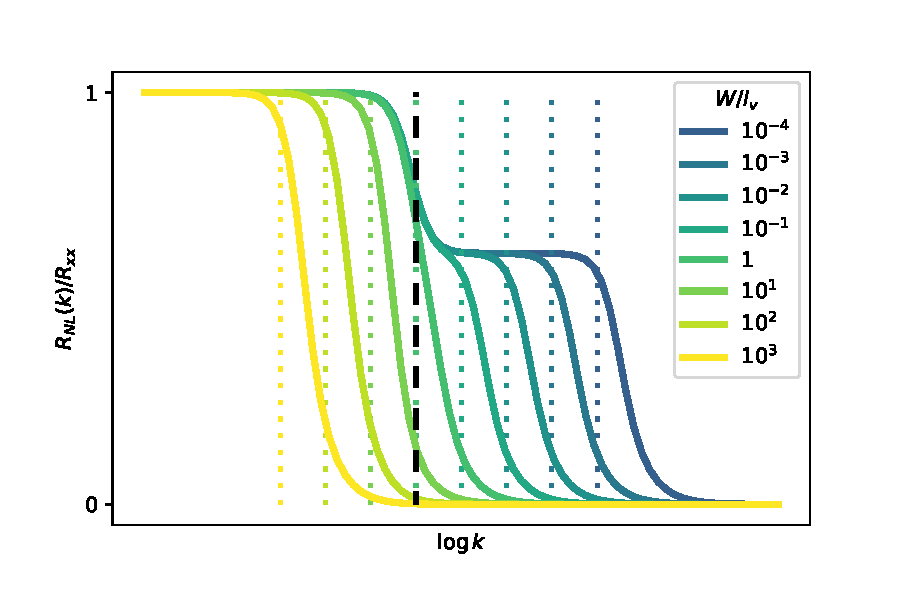
\includegraphics[width=\linewidth]{Immagini/rnl/widths.pdf}
    \caption{$R_{NK}(k)$ for several values of $W/l_\textrm{v}$. The dashed black line represents where $k=1/l_\textrm{v}$, the colored dashed line represents where $k=1/W$}
    \label{fig:RNLk}
\end{figure}
As you can see from the figure \ref{fig:RNLk} 
\begin{itemize}
    \item If $W\gg l_\textrm{v}$ we have a single bell like function with the width of the bell being $\approx 1/W$ and the height being $R_{xx}$ 
    \item If $W\ll l_\textrm{v}$ we have a double-bell function, where the first bell has a height of $R_{xx}$ and a width of $\approx 1/l_\textrm{v}$, and the second one has a shorter height.
\end{itemize}    
To evaluate the precise height of the secondary bell we just need to set $l_\textrm{v}^{-1}\ll k \ll W^{-1}$ in equation \ref{eq:rnlk}, this gives us

\begin{equation}
    R_{\textrm{NL}}(l_\textrm{v}^{-1}\ll k \ll W^{-1})\approx R_{xx}\cos^2(\theta_{\textrm{VH}})   
    \label{eq:plateau} 
\end{equation}
Where $R_{xx}=\frac{W}{\sigma_{xx}}$ and $\cos^2(\theta_{\textrm{VH}})=\frac{1}{1+\tan^2(\theta_{\textrm{VH}})}$

So, if we have $l_\textrm{v}\ll W$ or $\theta_{\textrm{VH}}\ll 1$ (or both) we have a single bell structure. Incidentally these are the conditions to NOT have topological effects, so the less visible the double bell is, the less visible the topological effects are. We'll also see later how one of the bell represents the ohmic nonlocal signal, while the other represents the topological nonlocal signal. 

\subsection{Small $k$}
Let's start by exploring $k\ll l_\textrm{v}^{-1},W^{-1}$. This will tell us how the function behaves at long ranges $x\gg l_\textrm{v},W$. In this regime 

\begin{equation}
    \omega(k)=\sqrt{k^2+l_\textrm{v}^{-2}}\approx \frac 1{l_\textrm{v}}\left[1+\frac{(kl_\textrm{v})^2}2\right]
\end{equation}
\begin{equation}
    \coth (kW/2)\approx \frac 2{kW} + \frac{kW}6
\end{equation}
Plugging the last two equations into equation \ref{eq:rnlk} we have that $R_{\textrm{NL}}(k)\approx$
\begin{equation}
    \frac 2{\sigma_c}\frac 1 {l_\textrm{v}k}\left[
        \frac 1{l_\textrm{v}}\left(1+\frac{k^2l_\textrm{v}^2}{2}\right)\left(\frac 2{kW} + \frac{kW}6\right)+
        \frac{k\tan^2(\theta_{\textrm{VH}})}{\tanh(W/2l_\textrm{v})} + o(k^2)
    \right]^{-1}
\end{equation}
And after some steps we get that
\begin{equation}
    R_{\textrm{NL}}(k\ll l_\textrm{v}^{-1},W^{-1})=
    \frac {R_{xx}}{1+L_\textrm{v}^2k^2 + o(k^4)}
    \label{eq:lorentz0}
\end{equation}
Where the \textit{renormalized valley diffusion length} $L_\textrm{v}^2$ is defined as
\begin{equation}
    L_\textrm{v}^2 \equiv l_\textrm{v}^2+\frac {W^2}{12} +\frac{l_\textrm{v}W}2 \frac{\tan^2(\theta_{\textrm{VH}})}{\tanh(W/2l_\textrm{v})}
\end{equation}
Now we are going to define the topological nonlocal resistance $R_{\textrm{NL}}^T$ by taking the equation \ref{eq:lorentz0}, and ignoring the $o(k^4)$ term
\begin{equation}
    R_{\textrm{NL}}^T(k)\equiv
    \frac {R_{xx}}{1+L_\textrm{v}^2k^2}
    \label{eq:lorentz1}
\end{equation} 
We are now ready to do the Fourier transform of equation \ref{eq:lorentz1} to get the behavior for $x\gg l_\textrm{v},W$
\begin{equation}
    R_{\textrm{NL}}(x\gg l_\textrm{v},W)\approx\mathcal F^{-1}\left[R_{\textrm{NL}}^T(k)\right]\equiv R_{\textrm{NL}}^T(x)
\end{equation}
That is equal to 

\begin{equation}
    R_{\textrm{NL}}^T(x)=
    R_{xx}\int_{-\infty}^{+\infty}
    \frac {e^{-ikx}}{1+L_\textrm{v}^2k^2}
    \frac {dk}{2\pi}=
    \frac{R_{xx}}{2L_\textrm{v}}e^{-\frac{|x|}{L_\textrm{v}}}
\end{equation}
So,
\begin{equation}
    R_{\textrm{NL}}(x\gg l_\textrm{v},W)\approx R_{\textrm{NL}}^T(x)
    \label{eq:rxg}
\end{equation}

\subsection{Big $k$}
Fortunately the case for which $k\gg l_\textrm{v}^{-1}$ is much simpler: in this case $\omega(k) \approx k$, so

\begin{equation}
    R_{\textrm{NL}}(k\gg l_\textrm{v}^{-1})=\cos^2(\theta_{\textrm{VH}})\frac {2\rho}{k}\tanh\left(\frac{kW}2\right)
\end{equation}
Using equation \ref{eq:ohmick} we get that this last equation is $\cos^2(\theta_{\textrm{VH}})$ times the one for the purely ohmic nonlocal signal
\begin{equation}
    R_{\textrm{NL}}(k\gg l_\textrm{v}^{-1})\approx
    \cos^2(\theta_{\textrm{VH}})R_{\textrm{NL}}^{(0)}(k)
\end{equation}
This means that the Fourier transform is
\begin{equation}
    R_{\textrm{NL}}(x\ll l_\textrm{v})\approx\cos^2(\theta_{\textrm{VH}})R_{\textrm{NL}}^{(0)}(x)
    \label{eq:rxl}
\end{equation}
\subsection{Testing the approximations}
But how do these equations fear in practice?
\begin{figure}[h!]
    \centering
    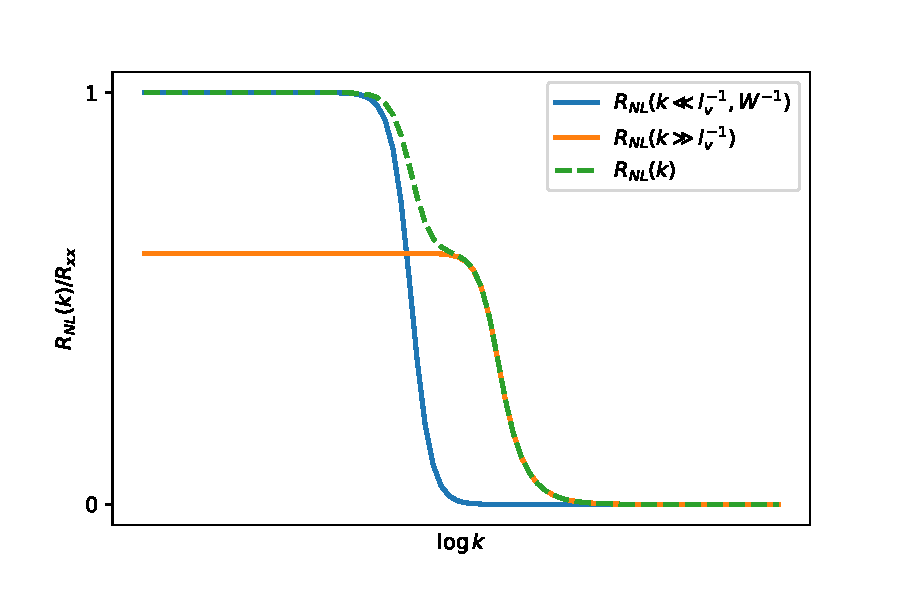
\includegraphics[width=\linewidth]{Immagini/rnl/2approx.pdf}
    \caption{For this example $l_\textrm{v}=20W$}
    \label{fig:rnl2approx}
\end{figure}
As you can see from figure \ref{fig:rnl2approx} the two approximations work pretty well, except in the neighborhood where $k\approx l_\textrm{v}^{-1}$. But what we really care about is $R_{\textrm{NL}}(x)$.\\
If we plot the approximations for $x\gg l_\textrm{v},W$ (eq. \ref{eq:rxg}) and $x\ll l_\textrm{v}$ (eq. \ref{eq:rxl}) alongside the numerical Fourier transform of $R_{\textrm{NL}}(k)$ \ref{eq:rnlk} we get figure \ref{fig:rnlx2approx}

\begin{figure}[h!]
    \centering
    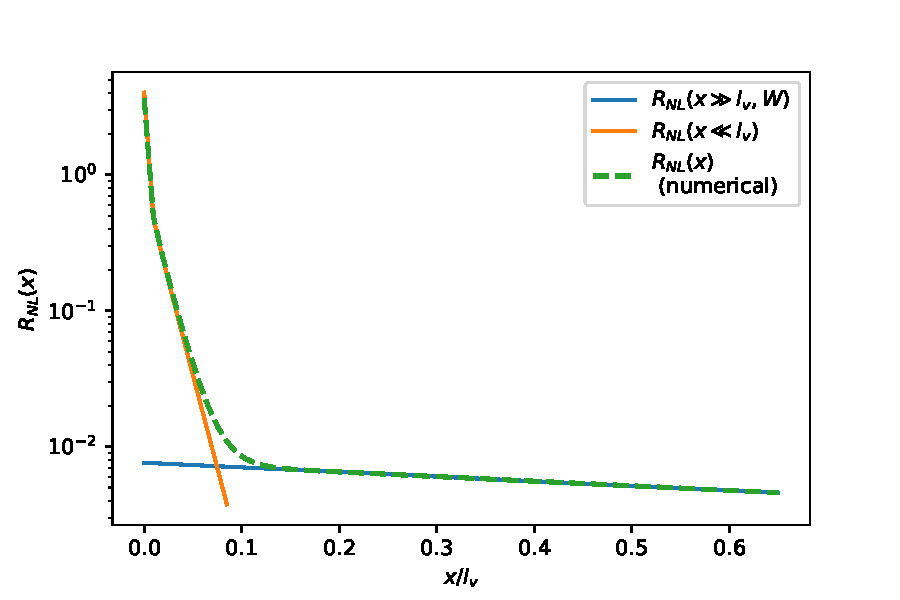
\includegraphics[width=\linewidth]{Immagini/rnl/x2approx.pdf}
    \caption{The parameters for this graph are exactly the same for the previous graph (figure \ref{fig:rnl2approx})}
    \label{fig:rnlx2approx}
\end{figure}
\subsection{Improving the approximation}
We can do better than this! By combining the two approximations it's possible to have a single equation that is very accurate for both $x\gg l_\textrm{v},W$ and $x\ll l_\textrm{v}$, however, in the end we'll end up with an approximation that is surprisingly good even for  $x\approx l_\textrm{v}$.

Since the Fourier transform is a linear operator, the idea is to find the linear combination of the two approximation that best approximates the $R_{\textrm{NL}}(k)$ for both $k\ll l_\textrm{v}^{-1},W^{-1}$ and $k\gg l_\textrm{v}^{-1}$ and then anti-transform the result.
\[
    R_{\textrm{NL}}(k)\approx \alpha R_{\textrm{NL}}(k\ll l_\textrm{v}^{-1},W^{-1}) +\beta R_{\textrm{NL}}(k\gg l_\textrm{v}^{-1})=
\]
\[
    =R_{\textrm{NL}}(k)\approx \alpha R_{\textrm{NL}}^T(k) +\beta\cos^2(\theta_{\textrm{VH}}) R_{\textrm{NL}}^{(0)}(k)      
\]
Where $\alpha$ and $\beta$ are the coefficient to be determined.\\
Since we only need to evaluate two variables, we only need to evaluate the expression above in two different points. The most reasonable points to choose are $k=0$ and $k=+\infty$, since they are the points where the approximations work better. For doing the calculations it's best to write out the two approximations 
\[
    R_{\textrm{NL}}(k)\approx 
    \alpha \frac {R_{xx}}{1+L_\textrm{v}^2k^2}+
    \beta\frac {2\rho}{k}\tanh\left(\frac{kW}2\right)\cos^2(\theta_{\textrm{VH}})
\]
\begin{itemize}
    \item For $k\to +\infty$ the term that is multiplied by $\beta$ is an increasingly precise estimate of $R_{\textrm{NL}}(k)$, and it dominates over the term that is multiplied by alpha, so $\beta=1$.
    \item For $k=0$ we have that
    \[
        R_{xx}=\alpha R_{xx} +  R_{xx}\cos^2(\theta_{\textrm{VH}})   
    \]
    So, $\alpha=\sin^2(\theta_{\textrm{VH}})$. 
\end{itemize}
Putting it all together we define the resulting approximation
\begin{equation}
    \boxed{
        \tilde R_{\textrm{NL}}(k)\equiv
        \sin^2(\theta_{\textrm{VH}})R_{\textrm{NL}}^{T}(k)+
        \cos^2(\theta_{\textrm{VH}})R_{\textrm{NL}}^{(0)}(k)
    }
\end{equation}
The thing that I personally like about this approximation is its geometrical elegance. If we write all the terms of the equation above we get
\begin{equation}
    \tilde R_{\textrm{NL}}(k)\equiv
    \sin^2(\theta_{\textrm{VH}})\frac {R_{xx}}{1+L_\textrm{v}^2k^2}+
    \cos^2(\theta_{\textrm{VH}})\frac {2\rho}{k}\tanh\left(\frac{kW}2\right)
\end{equation}
And if we plot the approximation $\tilde R_{\textrm{NL}}(k)$ alongside the actual values of $R_{\textrm{NL}}(k)$ we can see that they are remarkably similar (figure \ref{fig:kapproxcomp})
\begin{figure}[h!]
    \centering
    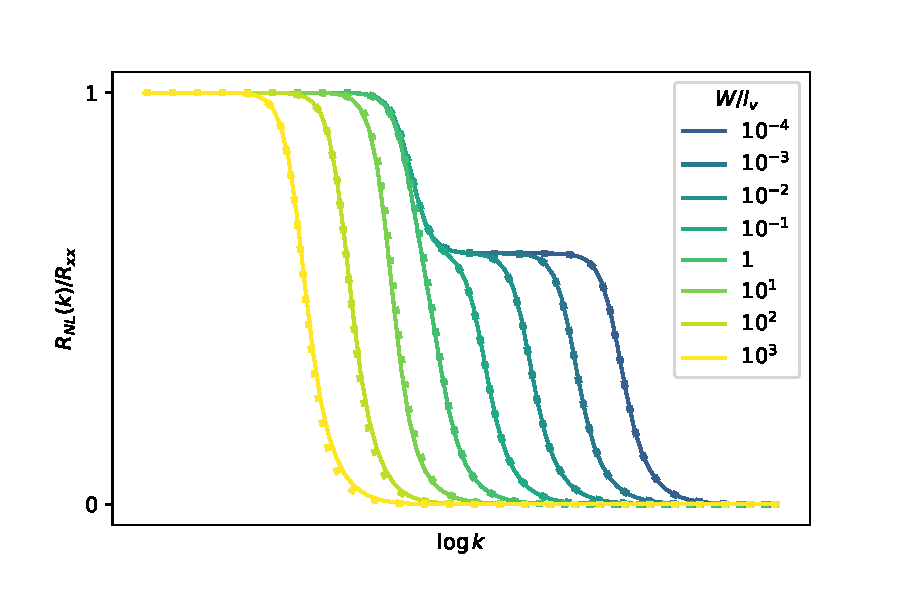
\includegraphics[width=\linewidth]{Immagini/rnl/kapproxcomp.pdf}
    \caption{Comparison between $R_{\textrm{NL}}(k)$ and $\tilde R_{\textrm{NL}}(k)$. The continuous line represents $R_{\textrm{NL}}(k)$, while the dashed line represents $\tilde R_{\textrm{NL}}(k)$. It's unreasonably accurate!}
    \label{fig:kapproxcomp}
\end{figure}\\
The nice thing about this is that if two equations are similar, then their Fourier transform will be too.
This means that $\tilde R_{\textrm{NL}}(x)$ will be a good approximation of $R_{\textrm{NL}}(x)$, where
\begin{equation}
    \boxed{
        \tilde R_{\textrm{NL}}(x)=
        \sin^2(\theta_{\textrm{VH}})R_{\textrm{NL}}^T(x)+
        \cos^2(\theta_{\textrm{VH}})R_{\textrm{NL}}^{(0)}(x)
    }
    \label{eq:rnl}
\end{equation}
We can write out the full formula using equations \ref{eq:rxg} and \ref{eq:rxl}
\begin{equation}
    \tilde R_{\textrm{NL}}(x)=
    \frac{R_{xx}}{2L_\textrm{v}}e^{-|x|/L_\textrm{v}}\sin^2(\theta_{\textrm{VH}})-
    \frac{2R_{xx}}{\pi W}\ln \bigg|\tanh \Big(\frac{\pi x}{2W}\Big)\bigg|\cos^2(\theta_{\textrm{VH}})
\end{equation}
Infact if we re-create figure \ref{fig:rnlx2approx} with the equation above we get figure \ref{fig:rnlxapprox}
\begin{figure}[h!]
    \centering
    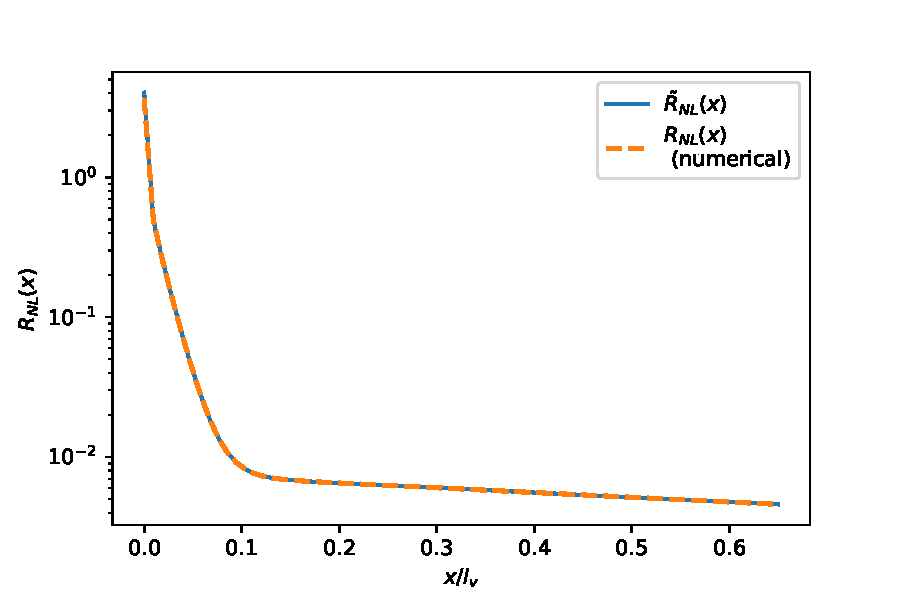
\includegraphics[width=\linewidth]{Immagini/rnl/xapprox.pdf}
    \caption{As you can see it's impossible to distinguish the difference between the two functions to the naked eye. The parameters are the same as figure \ref{fig:rnlxapprox}}
    \label{fig:rnlxapprox}
\end{figure}